\documentclass[11pt,preprint, authoryear]{elsarticle}

\usepackage{lmodern}
%%%% My spacing
\usepackage{setspace}
\setstretch{1.2}
\DeclareMathSizes{12}{14}{10}{10}

% Wrap around which gives all figures included the [H] command, or places it "here". This can be tedious to code in Rmarkdown.
\usepackage{float}
\let\origfigure\figure
\let\endorigfigure\endfigure
\renewenvironment{figure}[1][2] {
    \expandafter\origfigure\expandafter[H]
} {
    \endorigfigure
}

\let\origtable\table
\let\endorigtable\endtable
\renewenvironment{table}[1][2] {
    \expandafter\origtable\expandafter[H]
} {
    \endorigtable
}


\usepackage{ifxetex,ifluatex}
\usepackage{fixltx2e} % provides \textsubscript
\ifnum 0\ifxetex 1\fi\ifluatex 1\fi=0 % if pdftex
  \usepackage[T1]{fontenc}
  \usepackage[utf8]{inputenc}
\else % if luatex or xelatex
  \ifxetex
    \usepackage{mathspec}
    \usepackage{xltxtra,xunicode}
  \else
    \usepackage{fontspec}
  \fi
  \defaultfontfeatures{Mapping=tex-text,Scale=MatchLowercase}
  \newcommand{\euro}{€}
\fi

\usepackage{amssymb, amsmath, amsthm, amsfonts}

\def\bibsection{\section*{References}} %%% Make "References" appear before bibliography


\usepackage[round]{natbib}

\usepackage{longtable}
\usepackage[margin=2.3cm,bottom=2cm,top=2.5cm, includefoot]{geometry}
\usepackage{fancyhdr}
\usepackage[bottom, hang, flushmargin]{footmisc}
\usepackage{graphicx}
\numberwithin{equation}{section}
\numberwithin{figure}{section}
\numberwithin{table}{section}
\setlength{\parindent}{0cm}
\setlength{\parskip}{1.3ex plus 0.5ex minus 0.3ex}
\usepackage{textcomp}
\renewcommand{\headrulewidth}{0.2pt}
\renewcommand{\footrulewidth}{0.3pt}

\usepackage{array}
\newcolumntype{x}[1]{>{\centering\arraybackslash\hspace{0pt}}p{#1}}

%%%%  Remove the "preprint submitted to" part. Don't worry about this either, it just looks better without it:
\makeatletter
\def\ps@pprintTitle{%
  \let\@oddhead\@empty
  \let\@evenhead\@empty
  \let\@oddfoot\@empty
  \let\@evenfoot\@oddfoot
}
\makeatother

 \def\tightlist{} % This allows for subbullets!

\usepackage{hyperref}
\hypersetup{breaklinks=true,
            bookmarks=true,
            colorlinks=true,
            citecolor=blue,
            urlcolor=blue,
            linkcolor=blue,
            pdfborder={0 0 0}}


% The following packages allow huxtable to work:
\usepackage{siunitx}
\usepackage{multirow}
\usepackage{hhline}
\usepackage{calc}
\usepackage{tabularx}
\usepackage{booktabs}
\usepackage{caption}


\newenvironment{columns}[1][]{}{}

\newenvironment{column}[1]{\begin{minipage}{#1}\ignorespaces}{%
\end{minipage}
\ifhmode\unskip\fi
\aftergroup\useignorespacesandallpars}

\def\useignorespacesandallpars#1\ignorespaces\fi{%
#1\fi\ignorespacesandallpars}

\makeatletter
\def\ignorespacesandallpars{%
  \@ifnextchar\par
    {\expandafter\ignorespacesandallpars\@gobble}%
    {}%
}
\makeatother

\newlength{\cslhangindent}
\setlength{\cslhangindent}{1.5em}
\newenvironment{CSLReferences}%
  {\setlength{\parindent}{0pt}%
  \everypar{\setlength{\hangindent}{\cslhangindent}}\ignorespaces}%
  {\par}


\urlstyle{same}  % don't use monospace font for urls
\setlength{\parindent}{0pt}
\setlength{\parskip}{6pt plus 2pt minus 1pt}
\setlength{\emergencystretch}{3em}  % prevent overfull lines
\setcounter{secnumdepth}{5}

%%% Use protect on footnotes to avoid problems with footnotes in titles
\let\rmarkdownfootnote\footnote%
\def\footnote{\protect\rmarkdownfootnote}
\IfFileExists{upquote.sty}{\usepackage{upquote}}{}

%%% Include extra packages specified by user

%%% Hard setting column skips for reports - this ensures greater consistency and control over the length settings in the document.
%% page layout
%% paragraphs
\setlength{\baselineskip}{12pt plus 0pt minus 0pt}
\setlength{\parskip}{12pt plus 0pt minus 0pt}
\setlength{\parindent}{0pt plus 0pt minus 0pt}
%% floats
\setlength{\floatsep}{12pt plus 0 pt minus 0pt}
\setlength{\textfloatsep}{20pt plus 0pt minus 0pt}
\setlength{\intextsep}{14pt plus 0pt minus 0pt}
\setlength{\dbltextfloatsep}{20pt plus 0pt minus 0pt}
\setlength{\dblfloatsep}{14pt plus 0pt minus 0pt}
%% maths
\setlength{\abovedisplayskip}{12pt plus 0pt minus 0pt}
\setlength{\belowdisplayskip}{12pt plus 0pt minus 0pt}
%% lists
\setlength{\topsep}{10pt plus 0pt minus 0pt}
\setlength{\partopsep}{3pt plus 0pt minus 0pt}
\setlength{\itemsep}{5pt plus 0pt minus 0pt}
\setlength{\labelsep}{8mm plus 0mm minus 0mm}
\setlength{\parsep}{\the\parskip}
\setlength{\listparindent}{\the\parindent}
%% verbatim
\setlength{\fboxsep}{5pt plus 0pt minus 0pt}



\begin{document}



\begin{frontmatter}  %

\title{Helping You Write Academic Papers in R using Texevier}

% Set to FALSE if wanting to remove title (for submission)




\author[Add1]{Nico Katzke\footnote{\textbf{Contributions:} \newline \emph{The authors
  would like to thank no institution for money donated to this project.
  Thank you sincerely.}}}
\ead{nfkatzke@gmail.com}

\author[Add1,Add2]{John Smith}
\ead{John@gmail.com}

\author[Add1,Add2]{John Doe}
\ead{Joe@gmail.com}



\address[Add1]{Prescient Securities, Cape Town, South Africa}
\address[Add2]{Some other Institution, Cape Town, South Africa}

\cortext[cor]{Corresponding author: Nico Katzke\footnote{\textbf{Contributions:} \newline \emph{The authors
  would like to thank no institution for money donated to this project.
  Thank you sincerely.}}}

\begin{abstract}
\small{
Abstract to be written here. The abstract should not be too long and
should provide the reader with a good understanding what you are writing
about. Academic papers are not like novels where you keep the reader in
suspense. To be effective in getting others to read your paper, be as
open and concise about your findings here as possible. Ideally, upon
reading your abstract, the reader should feel he / she must read your
paper in entirety.
}
\end{abstract}

\vspace{1cm}

\begin{keyword}
\footnotesize{
Multivariate GARCH \sep Kalman Filter \sep Copula \\ \vspace{0.3cm}
\textit{JEL classification} L250 \sep L100
}
\end{keyword}
\vspace{0.5cm}
\end{frontmatter}



%________________________
% Header and Footers
%%%%%%%%%%%%%%%%%%%%%%%%%%%%%%%%%
\pagestyle{fancy}
\chead{}
\rhead{}
\lfoot{}
\rfoot{\footnotesize Page \thepage}
\lhead{}
%\rfoot{\footnotesize Page \thepage } % "e.g. Page 2"
\cfoot{}

%\setlength\headheight{30pt}
%%%%%%%%%%%%%%%%%%%%%%%%%%%%%%%%%
%________________________

\headsep 35pt % So that header does not go over title




\hypertarget{introduction}{%
\section{\texorpdfstring{Introduction
\label{Introduction}}{Introduction }}\label{introduction}}

path dependence; first rule of investment management

Due to the aforementioned sensitivity issues surrounding errors in the
expected return estimation, this work will only cover the portfolio
optimisation techniques that intentionally forego this input. These
include the naive equal weight, inverse variance, hierarchical risk
parity, ERC and the minimum variance portfolios. \emph{The theoretical
underpinnings of each will be reviewed as well as their relative
performance in historical back tests}.

``. Markowitz's curse is that the more correlated investments are, the
greater is the need for a diversified portfolio---and yet the greater
are that portfolio's estimation errors. (De Prado,
\protect\hyperlink{ref-lopez}{2016})''

\hypertarget{aims-and-objectives}{%
\section{Aims and Objectives}\label{aims-and-objectives}}

This work aims to use Monte Carlo Methods to uncover the relationship
between a market's covariance structure and the risk return properties
of various portfolio optimisation algorithms. This will be achieved
through the following objectives.

\begin{enumerate}
\def\labelenumi{\arabic{enumi}.}
\item
  Design and create five distinct \emph{ad hoc} \emph{20 by 20}
  correlation matrices, each corresponding to a different risk structure
  or market type. These will range from a structure possessing no
  clusters to those possessing hierarchical clustering.
\item
  Use the R package \emph{MCmarket} to perform Monte Carlo Simulations
  for each of the five \emph{ad hoc} correlation matrices {[}REFERENCE
  MYSELF{]}. The markets will be designed to have student t multivariate
  distributions, with 3 degrees of freedom, the returns will each be
  univariate normally distributed with a periodic mean of 0.02 and
  standard deviation of 0.1. Each market type will be simulated 10 000
  times across 300 periods.
\item
  Use the simulated markets to calculate the returns obtained from the
  portfolio optimisers. The first 50 periods will be used estimate the
  \emph{ex ante} covariance matrix and the portfolio returns will be
  calculated on the remaining 250 periods. (should properly incorporate
  rebalancing!!!!!!! every 50 periods?). The
\item
  The performance of each portfolio optimiser will then be compared and
  contrasted using various portfolio risk/return analytics. Portfolio
  optimisers will be compared with each other within market types and
  with themselves across markets types.
\end{enumerate}

\hypertarget{litrature-review}{%
\section{Litrature Review}\label{litrature-review}}

\hypertarget{a-review-of-portfolio-optimisation-algorithms}{%
\subsection{A Review of Portfolio Optimisation
Algorithms}\label{a-review-of-portfolio-optimisation-algorithms}}

\hypertarget{introduction-1}{%
\subsubsection{Introduction}\label{introduction-1}}

Since Harry Markovitz's (1952) seminal work on the mean-variance
portfolios scholars from around the globe have been aspiring to develop
a robust algorithm capable of \emph{ex ante} situating a portfolio on
the efficient frontier (Markowitz,
\protect\hyperlink{ref-markowitz}{1952}). There are now a wide array of
available alternatives portfolio optimisers. They range from simple
heuristic based approaches to advanced mathematical algorithms based on
quadratic optimisation, random matrix theory and machine learning
methods; many more are still in the making.

These optimisers however are not without their flaws. Mean-variance
optimisers, in particular, rely heavily on the accuracy of return
forecasts, where small changes in the expected return input can lead to
large changes in portfolio weights (De Prado,
\protect\hyperlink{ref-lopez}{2016}). Due to this issue only so-called
risk based portfolio's that intentionally avoid using expected return
forecasts are discussed in this work as they are said to be more robust
to estimation error (Maillard,
\protect\hyperlink{ref-maillard2010}{2010}). Furthermore, quadratic
programming methods used in portfolio optimisation require the inversion
of some positive-definite covariance matrix, which can be susceptible to
error if the covariance matrix suffers from a high condition number.
where a condition number is defined as the absolute value of the ratio
between a covariance matrix's largest and smallest eigenvalues (Bailey
\& Lopez De Prado, \protect\hyperlink{ref-lopez2012}{2012}; De Prado,
\protect\hyperlink{ref-lopez}{2016}). Diagonal matrices have the
smallest condition number which increases as more correlated variables
are added. When working with high conditional number matrices a small
change in a single entry's estimated covariance can greatly alter its
inverse of, which in turn can effect the portfolio weights (De Prado,
\protect\hyperlink{ref-lopez}{2016}). This is exacerbated by the fact
that covariance matrices themselves are prone to estimation error. For a
given sample size, larger dimension co-variance matrices are prone to
more noise in estimation. This is essentially due to a reduction in
degrees of freedom as a sample of at least \(1/2N(N+1)\) independent and
identically distributed (iid) observations are required to estimate an
\(N\times N\) covariance matrix. Furthermore, financial market
covariance structures tend to vary over time and have been know to
change rapidly during so-called regime changes (De Prado,
\protect\hyperlink{ref-lopez}{2016}). \textbf{{[}Regime changes{]}}

\hypertarget{naive-equal-weight-ew}{%
\subsubsection{Naive Equal Weight (EW)}\label{naive-equal-weight-ew}}

Perhaps the oldest and most simple portfolio diversification heuristic
constitutes holding a weight of \(1/N\) of the \(N\) total assets
available to the investor (DeMiguel \emph{et al.},
\protect\hyperlink{ref-demiguel2009}{2009}). This portfolio is commonly
called the equal weight or 1/N portfolio, its failure to recognise the
importance of covariation between assets has resulted in it also being
referred to as the naive portfolio. It commonly used as a benchmark
index.

Despite its simplistic nature empirical studies tend to find a
statistically insignificant difference in Sharp ratio between the naive
portfolio and more advanced portfolio optimisers. This finding was made
in DeMiguel \emph{et al.} (\protect\hyperlink{ref-demiguel2009}{2009})
who looked at the mean-variance, minimum-variance and Bayes-Stein
portfolio's, where EW also performed surprisingly well form a total
return perspective.

\hypertarget{minimum-variance-mv}{%
\subsubsection{Minimum Variance (MV)}\label{minimum-variance-mv}}

Portfolio optimisers designed to exhibit the minimum variance have
garnered a lot of attention for themselves, largely to their tendency to
achieve surprisingly high returns in historical back tests (Clarke
\emph{et al.}, \protect\hyperlink{ref-clarke2011}{2011}). This
performance has been attributed to the fact that low volatility stocks
tend to earn returns in excess of the market, and high beta stocks tend
not to be rewarded by higher returns (Clarke \emph{et al.},
\protect\hyperlink{ref-clarke2011}{2011}; Fama \& French,
\protect\hyperlink{ref-fama1992}{1992}). These minimum variance
portfolios tend to achieve cumulative returns equal to or slightly
greater than market capitalization weighted portfolio's whilst
maintaining consistently lower variance and achieving a noticeable
improvement in downside risk mitigation even during times of financial
crisis (Clarke \emph{et al.}, \protect\hyperlink{ref-clarke2011}{2011}).
\textbf{The MV portfolio (discussed in this section) is the only
portfolio on the efficient frontier that does not depend on expected
return forecasts(De Prado, \protect\hyperlink{ref-lopez}{2016}).}

The minimum variance portfolio selects security weights such that the
resulting portfolio weights correspond to the portfolio with the lowest
possible in sample volatility. Therefore, it has the lowest expected
volatility and is, in theory, safest/least risky portfolio (De Carvalho
\emph{et al.},
\protect\hyperlink{ref-rawl2012}{2012}\protect\hyperlink{ref-rawl2012}{a}).
Its primary input is a variance covariance matrix, which it uses in its
optimisation to overweight low volatility and low correlation securities
(De Carvalho \emph{et al.},
\protect\hyperlink{ref-rawl2012}{2012}\protect\hyperlink{ref-rawl2012}{a}).
This approach often works well out of sample, but is known to achieve
minor reductions in \emph{ex ante} portfolio volatility by greatly
favouring a small number of low volatility/correlation securities (De
Prado, \protect\hyperlink{ref-lopez}{2016} {[}p.~68{]}). This tendency
to produce highly concentrated portfolio's can cause serious out of
sample diversification problem as the sample becomes increasingly
susceptible to measurement error.

Let \(\sum\) indicate the markets variance covariance matrix and
\(w=\{w_i,..., w_N \}\) be a vector of length N containing individual
security weights, then the vector containing MV portfolio can be written
as (De Carvalho \emph{et al.},
\protect\hyperlink{ref-rawl2012}{2012}\protect\hyperlink{ref-rawl2012}{a}):

\(w^*=arg\min(w'\sum w)\ \ \ s.t.\ \sum^N_iw_i=1\)

\hypertarget{inverse-varience-iv-weighting}{%
\subsubsection{Inverse-Varience (IV)
Weighting}\label{inverse-varience-iv-weighting}}

\textbf{The inverse-variance (IV), equal risk contrition (ERC) and
maximum diversification (MD) portfolio's each assume that adequate
diversification can be obtained by allocating equal risk to each
investable security.}

The IV portfolio, also known as the equal-risk budget (ERB), portfolio
aims to allocate an equal risk budget to each investable security (De
Carvalho \emph{et al.},
\protect\hyperlink{ref-leote}{2012}\protect\hyperlink{ref-leote}{b}).
Where the risk budget is defined as the the product of a the security's
weight and volatility. Therefore, if we define \(\sigma_i\) as security
i's volatility, then marginal volatility is equally distributed across N
securities by setting security weights as such:

\(w_{iv}=(\frac{1/\sigma_1}{\sum^N_{j=1} 1/\sigma}, ...,\frac{1/\sigma_N}{\sum^N_{j=1} 1/\sigma} )\)

\hypertarget{equal-risk-contribution-erc}{%
\subsubsection{Equal Risk Contribution
(ERC)}\label{equal-risk-contribution-erc}}

The ERC portfolio is similar to the IV, but also takes covariance into
account (De Carvalho \emph{et al.},
\protect\hyperlink{ref-leote}{2012}\protect\hyperlink{ref-leote}{b}).
The basic idea behind the ERC is to weight the portfolio such that each
security contributes equally to risk, which in turn maximises risk
diversification (Maillard, \protect\hyperlink{ref-maillard2010}{2010}).
Generally speaking the ERC acts similar to a weight constrained minimum
variance portfolio, with constraints ensuring that adequate
diversification is maintained. The weights of the ERC portfolio
\(x=(x_1,x_2,...,x_n)\) consisting of n assets is calculated as follows.

let \(\sigma_i^2\) resemble asset i's variance, \(\sigma_{ij}\) the
covariance between asset i and j and \(\sum\) be the markets variance
covariance matrix. Portfolio risk can now be written as
\(sigma(x)=\sqrt{x^T\sum x}=\sum_i\sum_{j\neq i}x_ix_j\sigma_{ij}\)
(Maillard, \protect\hyperlink{ref-maillard2010}{2010}). The marginal
risk contribution \(\partial_{x_i}\sigma(x)\) can then be defined as
follows (Maillard, \protect\hyperlink{ref-maillard2010}{2010}):

\(\partial_{x_i}\sigma(x)=\frac{\partial\sigma(x)}{\partial x_i}=\frac{x_i\sigma_i^2+\sum_{j\neq i}x_j\sigma_{ij}}{\sigma(x)}\)

Therefore, \(\partial_{x_i}\sigma(x)\) refers to the change in portfolio
volatility resulting from a small change in asset i's weight. ERC uses
this definition to guide its algorithms central objective to equate the
risk contribution for each asset in the portfolio \emph{ex ante}. If we
define \((\sum x)_i\) as the \(i^{th}\) row resulting from the product
of \(\sum\) with x and note that \(\partial_{x_i}\sigma(x)=(\sum x)_i\),
then the optimal ERC weight can be written as (Maillard,
\protect\hyperlink{ref-maillard2010}{2010}):

\(x^*=\{x \ \epsilon[0,1]^n:\sum x_i=1, x_i \times (\sum x)_i=x_j \times (\sum x)_j \ \forall \ i,j \}\)

\hypertarget{maximum-diversification-md}{%
\subsubsection{Maximum Diversification
(MD)}\label{maximum-diversification-md}}

Choueifaty \& Coignard (\protect\hyperlink{ref-choueifaty2008}{2008})
originally designed the MD portfolio to maximize the diversification
ratio (DR), which they defined as the as the sum of each securities risk
bucket divided by portfolio volatility (De Carvalho \emph{et al.},
\protect\hyperlink{ref-leote}{2012}\protect\hyperlink{ref-leote}{b}). If
we define \(w=(w_1,...w_N)^T\) as a vector of portfolio weights, V as a
vector of asset volatilities and \(\sum\) as the covariance matrix. Then
the DR can be expresses as:

\(DR= \frac{w'.V}{\sqrt{w'Vw}}\)

Therefore, much like the IV and ERC portfolio's, the MD portfolio
attempts to diversify the portfolio by allocating equal risk to each
security (Choueifaty \& Coignard,
\protect\hyperlink{ref-choueifaty2008}{2008}). The MD portfolio
accomplishes this by over-weighting low volatility securities and those
that are less correlated with other stocks (De Carvalho \emph{et al.},
\protect\hyperlink{ref-leote}{2012}\protect\hyperlink{ref-leote}{b}).
For detail regarding the theoretical results and properties of the MD
portfolio see Choueifaty \& Coignard
(\protect\hyperlink{ref-choueifaty2008}{2008}: 33--35).

`The MD strategy, introduced by Choueifaty and Coignard {[}2008{]},
invests in the portfolio that maximizes a diversification ratio. The
ratio is the sum of the risk budget allocated to each stock in the
portfolio divided by the portfolio volatility. This strategy should
invest in stocks that are less correlated to other stocks.' (copy
pasted)

\hypertarget{empirical-backtests}{%
\subsection{Empirical Backtests}\label{empirical-backtests}}

Choueifaty \emph{et al.} (\protect\hyperlink{ref-choueifaty2013}{2013})
conducted an empirical back test comparing the relative performance if
numerous portfolio optimisers between 1999 and 2010. They used
historical data from the MSCI World world index and considered the
largest 50\% of assets at each semi-annual rebalance date. At each
rebalance date the covariance matrices, used as inputs in the portfolio
optimisers, were estimated using the passed years worth of data
(Choueifaty \emph{et al.},
\protect\hyperlink{ref-choueifaty2013}{2013}). This was done to reduce
noise in estimation. All portfolio's were restricted to long only. The
MV portfolio achieved an annual return of 6.7\% and outperformed the ERC
and EW portfolio's who returned 6.3\% and 5.8\% respectively.
Unsurprisingly, the MV portfolio possessed the lowest daily volatility
(10\%) followed by the ERC and then the EW portfolio's (with 12.9\% and
16.4\% respectively). Accordingly the MV portfolio scored the highest
sharp ratio (0.36) followed by the ERC and EW portfolio's (0.24 and 0.16
respectively).

\hypertarget{hierarchical-risk-parity-hrp}{%
\subsubsection{Hierarchical Risk Parity
(HRP)}\label{hierarchical-risk-parity-hrp}}

Due to the multitude of robustness issues related to traditional
portfolio optimisers, De Prado (\protect\hyperlink{ref-lopez}{2016})
developed a new approach incorporating machine-learning methods and
graph theory ({\textbf{???}}). De Prado
(\protect\hyperlink{ref-lopez}{2016}) argues that the ``lack of
hierarchical structure in a correlation matrix allows weights to vary
freely in unintended ways'' and that this contributes to the instability
issues. His HRP algorithm requires only a singular co-variance matrix
and can utilize the information within without the need for the positive
definite property (De Prado, \protect\hyperlink{ref-lopez}{2016}). This
procedure works in three stages:

De Prado (\protect\hyperlink{ref-lopez}{2016}) carried out an in sample
simulation study comparing the respective allocations of the long-only
minimum variance, IVP and HRP portfolios using a co-variance matrix
using a condition number that is ``not unfavourable'' to the minimum
variance portfolio. The simulated data consisted of 10000 observations
across 10 variables. The following findings were made: The minimum
variance portfolio concentrated 92.66\% of funds in the top 5 holdings
and assigned a zero weight to 3 assets. \emph{Conversly}, HRP only
assigned 62.5\% of its funds to the top 5 holdings (De Prado,
\protect\hyperlink{ref-lopez}{2016}). The minimum variance portfolio's
objective function causes it to build highly concentrated portfolio's in
favor of a small reduction in volatility; the HRP portfolio had only a
slightly higher volatility (De Prado,
\protect\hyperlink{ref-lopez}{2016}). This apparent diversification
advantage achieved by the minimum variance portfolio is rather deceptive
as the portfolio remains highly susceptible to idiosyncratic risk
incidents within its top holdings (De Prado,
\protect\hyperlink{ref-lopez}{2016}). This claim was further validated
by the finding that HRP achieved significantly lower out of sample
variance compared to the minimum variance portfolio.

\hypertarget{methadology}{%
\section{Methadology}\label{methadology}}

This work used Monte Carlo simulation methods to investigate the link
between a markets correlation structure and the relative performance of
the EW, MV, IV, ERC and MD portfolios. The following may become
confusing so please note the following terminology. In this study the
term market can be thought of as a single observation consisting of the
daily returns for a number of assets, where market type refers to an
ensemble of markets each designed to posses the same characteristics.
Here the ensemble units are referred to as realizations or
counterfactuals.

The R package MCmarket was used to simulate five distinctive market
types, each with 300 periods of returns, 20 assets and 10 000
realizations. Each market type was was designed, \emph{ad hoc}, to
posses a unique correlation structure. These structures range from a
matrices with no correlation (i.e.~a diagonal matrix) to those with
possessing hierarchical clustering (see \ref{corr_struc})
({\textbf{???}}).

The EW, MV, IV, ERC and MD portfolios were then backtested on the
simulated markets. The first 50 periods, of each realisation, was used
to estimate a 20 by 20 co-variance matrix, used as the primary input in
calculating the weights for the respective portfolios. These weights
were then used in conjunction with the simulated returns to calculate
the returns for the respective portfolios.

Portfolio analytics are then performed for each portfolio type on each
realization within the market types. These portfolio analytics include
the standard deviation (sd) of daily returns, downside deviation, value
at risk (VaR), conditional VAR (CVaR), Sharp ratio, average drawdown and
maximum drawdown. The mean and median of the portfolio metrics are then
calculated for each market type.

Finally, the portfolio metrics are compared within portfolio types
across market types and within market types across portfolio types.

\hypertarget{correlation-structures}{%
\subsection{\texorpdfstring{Correlation Structures
\label{corr_struc}}{Correlation Structures }}\label{correlation-structures}}

\hypertarget{ad-hoc}{%
\subsubsection{\texorpdfstring{\emph{Ad Hoc}}{Ad Hoc}}\label{ad-hoc}}

Figure \ref{corr_mats} presents the four \emph{ad hoc} correlation
matrices used in this study.

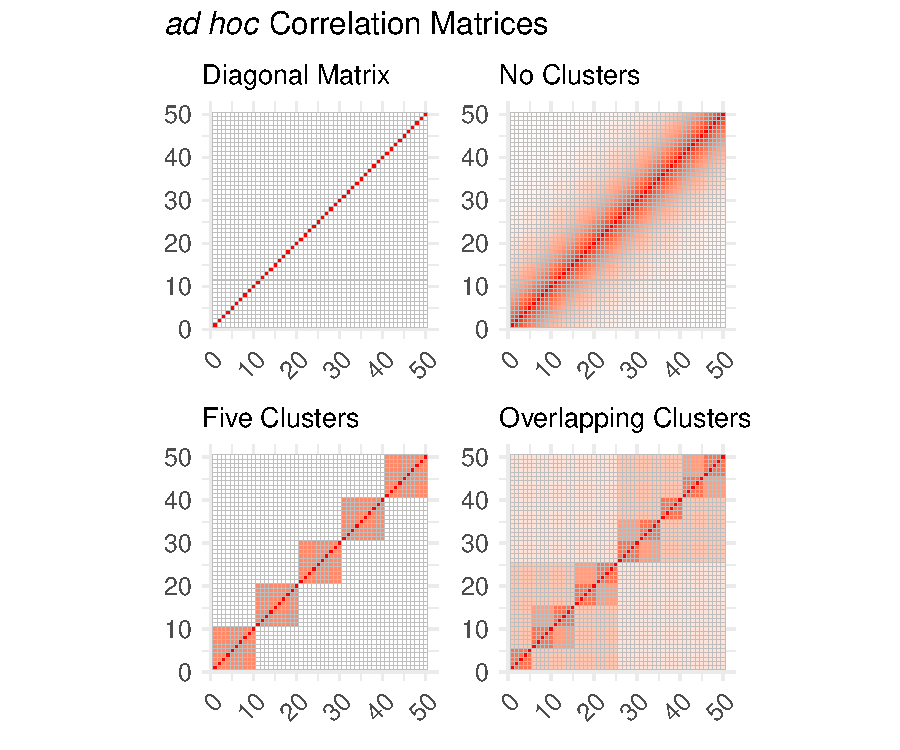
\includegraphics{Thesis_files/figure-latex/corr mats-1.pdf} \#\#\#
Emperical

\hypertarget{monte-carlo}{%
\subsection{Monte Carlo}\label{monte-carlo}}

\hypertarget{back-tests}{%
\subsection{Back Tests}\label{back-tests}}

\hypertarget{portfolio-analytics}{%
\subsection{Portfolio Analytics}\label{portfolio-analytics}}

\hypertarget{results-and-discussion}{%
\section{Results and Discussion}\label{results-and-discussion}}

\hypertarget{conclusion}{%
\section{Conclusion}\label{conclusion}}

I hope you find this template useful. Remember, stackoverflow is your
friend - use it to find answers to questions. Feel free to write me a
mail if you have any questions regarding the use of this package. To
cite this package, simply type citation(``Texevier'') in Rstudio to get
the citation for Katzke (\protect\hyperlink{ref-Texevier}{2017}) (Note
that uncited references in your bibtex file will not be included in
References).

\newpage

\hypertarget{references}{%
\section*{References}\label{references}}
\addcontentsline{toc}{section}{References}

\hypertarget{refs}{}
\leavevmode\hypertarget{ref-lopez2012}{}%
Bailey, D.H. \& Lopez De Prado, M. 2012. Balanced baskets: A new
approach to trading and hedging risks. \emph{Journal of Investment
Strategies (Risk Journals)}. 1(4).

\leavevmode\hypertarget{ref-choueifaty2008}{}%
Choueifaty, Y. \& Coignard, Y. 2008. Toward maximum diversification.
\emph{The Journal of Portfolio Management}. 35(1):40--51.

\leavevmode\hypertarget{ref-choueifaty2013}{}%
Choueifaty, Y., Froidure, T. \& Reynier, J. 2013. Properties of the most
diversified portfolio. \emph{Journal of investment strategies}.
2(2):49--70.

\leavevmode\hypertarget{ref-clarke2011}{}%
Clarke, R., De Silva, H. \& Thorley, S. 2011. Minimum-variance portfolio
composition. \emph{The Journal of Portfolio Management}. 37(2):31--45.

\leavevmode\hypertarget{ref-rawl2012}{}%
De Carvalho, R.L., Lu, X. \& Moulin, P. 2012a. Demystifying equity
risk--based strategies: A simple alpha plus beta description. \emph{The
Journal of Portfolio Management}. 38(3):56--70.

\leavevmode\hypertarget{ref-leote}{}%
De Carvalho, R.L., Lu, X. \& Moulin, P. 2012b. Demystifying equity
risk--based strategies: A simple alpha plus beta description. \emph{The
Journal of Portfolio Management}. 38(3):56--70.

\leavevmode\hypertarget{ref-demiguel2009}{}%
DeMiguel, V., Garlappi, L. \& Uppal, R. 2009. Optimal versus naive
diversification: How inefficient is the 1/n portfolio strategy?
\emph{The review of Financial studies}. 22(5):1915--1953.

\leavevmode\hypertarget{ref-lopez}{}%
De Prado, M.L. 2016. Building diversified portfolios that outperform out
of sample. \emph{The Journal of Portfolio Management}. 42(4):59--69.

\leavevmode\hypertarget{ref-fama1992}{}%
Fama, E.F. \& French, K.R. 1992. The cross-section of expected stock
returns. \emph{the Journal of Finance}. 47(2):427--465.

\leavevmode\hypertarget{ref-Texevier}{}%
Katzke, N.F. 2017. \emph{Texevier: Package to create elsevier templates
for rmarkdown}. ed. Stellenbosch, South Africa: Bureau for Economic
Research.

\leavevmode\hypertarget{ref-maillard2010}{}%
Maillard, T., Roncalli. 2010. The properties of equally weighted risk
contribution portfolios. \emph{The Journal of Portfolio Management}.
36(4):60--70.

\leavevmode\hypertarget{ref-markowitz}{}%
Markowitz, H. 1952. Portfolio selection. \emph{The Journal of Finance}.
7(1):77--91.

\newpage

\hypertarget{appendix}{%
\section*{Appendix}\label{appendix}}
\addcontentsline{toc}{section}{Appendix}

\hypertarget{appendix-a}{%
\subsection*{Appendix A}\label{appendix-a}}
\addcontentsline{toc}{subsection}{Appendix A}

Some appendix information here

\hypertarget{appendix-b}{%
\subsection*{Appendix B}\label{appendix-b}}
\addcontentsline{toc}{subsection}{Appendix B}

\bibliography{Tex/ref}





\end{document}
